\documentclass[11pt,a4paper]{article}

\usepackage[a4paper,left=1.35in,right=1.35in,top=1.25in,bottom=1.05in]{geometry}
\usepackage{times}
\usepackage{setspace}
\usepackage{graphicx}
\usepackage{array}
\usepackage{booktabs}
\usepackage{longtable}
\usepackage{tabularx}
\usepackage{enumitem}
\usepackage{float}
\usepackage{caption}
\usepackage{hyperref}
\usepackage{xcolor}
\usepackage{tikz}
\usepackage{titlesec}
\usetikzlibrary{arrows.meta,positioning,shapes.geometric}

\hypersetup{
    colorlinks=true,
    linkcolor=black,
    citecolor=black,
    urlcolor=black,
    pdftitle={Site Meeting Copilot v2 Research Paper},
    pdfauthor={Kalla Lokaditya}
}

\setstretch{1.08}
\setlength{\parindent}{17pt}
\setlength{\parskip}{4pt}
\sloppy

\titleformat{\section}
  {\normalfont\Large\bfseries}{\thesection}{1em}{}
\titleformat{\subsection}
  {\normalfont\large\bfseries}{\thesubsection}{1em}{}
\titleformat{\subsubsection}
  {\normalfont\normalsize\bfseries}{\thesubsubsection}{1em}{}
\captionsetup{font=small,labelfont=bf}

\newcolumntype{Y}{>{\raggedright\arraybackslash}X}

\begin{document}

\begin{center}
    \vspace*{1.1cm}
    {\LARGE\bfseries A Local AI Framework for Construction Site Meeting Minutes Generation Using Whisper Transcription and Structured LLM Analysis\par}
    \vspace{1.0cm}
    {\large Kalla Lokaditya$^{1*}$\par}
    \vspace{0.55cm}
    {$^{1}$Department of Computer Science and Engineering, Dayananda Sagar University, Bengaluru, Karnataka, India.\par}
    \vspace{0.25cm}
    {*Corresponding author. USN: ENG23CS0570. E-mail: ENG23CS0570@dsu.edu.in\par}
\end{center}

\vspace{1.1cm}

\begin{center}
    \textbf{Abstract}
\end{center}

\noindent Construction site meetings produce important decisions, blockers, responsibilities, due dates, safety observations and schedule changes. In many small and medium construction projects, this evidence is captured as unstructured audio, handwritten notes, messaging app updates or spreadsheet revisions. Manual preparation of meeting minutes and action trackers is time consuming, and missing a single dependency can delay procurement, site execution or client communication. This paper presents Site Meeting Copilot v2, a local AI-based framework that converts construction site meeting evidence into structured and reviewable project governance outputs. The system accepts meeting audio or pasted transcript text, agenda text and a project schedule CSV. A local Flask Whisper server transcribes supported audio files, while Ollama with the phi3:mini language model analyses the transcript with agenda and schedule context. The framework extracts summaries, decisions, blockers, risks, action items, owners, due dates, agenda coverage and schedule impact flags. Outputs are displayed in a browser dashboard and can be exported as meeting minutes, an action tracker and a schedule impact report. The Version 1 implementation was evaluated using functional tests for audio upload, transcription server health, malformed schedule input, agenda matching, JSON extraction and report generation. The results show that a local AI pipeline can support site engineers by transforming unstructured meeting discussions into actionable project records while keeping the human user in control of review and approval.

\newpage

\noindent\textbf{Keywords:} Construction Site Meetings, Meeting Minutes, Automatic Speech Recognition, Whisper, Local Large Language Models, Ollama, Action Tracker, Schedule Impact Analysis, Project Governance, Construction AI.

\section{Introduction}

Construction projects depend on repeated coordination among owners, project managers, site engineers, consultants, contractors, suppliers and safety teams. Site meetings are used to review progress, identify blockers, approve decisions, assign responsibilities and resolve dependencies between work packages. Although these meetings are operationally important, the records generated during them are often incomplete or scattered across multiple informal sources. A single project decision may appear in a meeting recording, a WhatsApp message, an Excel schedule, a site diary and a later follow-up call. This fragmentation makes it difficult for teams to maintain a reliable project memory.

The preparation of meeting minutes is therefore an important but time-consuming activity. A site engineer may attend the meeting, make notes, inspect drawings, verify the schedule and later prepare a minutes of meeting document. If the meeting is long or contains many stakeholders, action items can be missed. If the schedule impact is not identified early, the project team may discover delays only after downstream work has already been affected. This problem is especially relevant in construction, where delayed materials, safety observations, access constraints, manpower shortages and blocked work fronts can quickly affect linked activities.

Recent progress in automatic speech recognition and local language models makes it possible to support this workflow using AI. Whisper-style transcription can convert audio into text, while compact language models can extract structured fields from the transcript. However, a normal meeting summarizer is not sufficient for a construction site workflow. A site meeting system should not simply produce a paragraph summary. It should identify decisions, blockers, owners, deadlines, agenda coverage and potential schedule impact. It should also allow the user to review the transcript and generated outputs because construction decisions require accountability.

Site Meeting Copilot v2 applies these capabilities to the construction meeting domain. The system works as a local prototype that accepts meeting audio or transcript text, agenda text and a project schedule CSV. It performs transcription using a local Whisper server, analyses the meeting using a local language model through Ollama, and renders structured outputs in a browser dashboard. The project is intended as a Version 1 release of a construction meeting intelligence assistant. It focuses on converting a meeting into reliable records: meeting minutes, action tracker entries and schedule impact indicators.

The contribution of this paper is an integrated framework for local construction meeting intelligence. The framework links local transcription, structured LLM extraction, agenda cross-reference checking and schedule impact analysis in a single workflow. The design keeps the transcript editable and the outputs reviewable because AI-generated meeting records should support a site engineer rather than replace professional judgement. The paper also maps the implemented features to Version 1 requirements and discusses how the same project can evolve into a larger construction AI operating system.

\section{Background and Related Work}

\subsection{Meeting Documentation in Construction Projects}

Meetings are a core communication mechanism in construction management. They are used to review progress, approve work, discuss technical issues, coordinate subcontractors and document responsibilities. Formal meeting minutes provide evidence of decisions and help prevent disputes. However, the quality of minutes depends on the person recording them, the time available after the meeting and the clarity of the discussion. In student projects and small organizations, meeting records are often prepared manually and may not include complete action ownership.

Construction meetings differ from generic business meetings because they are closely connected to the schedule, site constraints, material delivery, safety compliance and work package dependencies. For example, a discussion about delayed steel delivery is not only a procurement issue. It may affect column casting, formwork removal, slab work and labour allocation. Similarly, a safety observation may stop work until a corrective action is completed. Therefore, a construction meeting assistant must identify not only what was discussed, but also how it affects project execution.

\subsection{Automatic Speech Recognition}

Automatic speech recognition is the first layer of the proposed framework. Whisper demonstrated that models trained with large-scale weak supervision can generalize across varied speech conditions and convert audio recordings into text. The faster-whisper implementation uses CTranslate2 to support efficient local transcription. This makes it practical for a student prototype to run speech recognition on a local machine rather than relying entirely on cloud services.

In the proposed system, the Whisper server is exposed as a local Flask service. The frontend sends an uploaded audio file to the server, and the server returns a transcript. The transcript remains visible to the user so that errors can be corrected before AI analysis. This is important because noisy construction audio, overlapping speakers and domain-specific names can introduce transcription mistakes.

\subsection{Local Language Models}

Large language models are useful for extracting structured information from unstructured text. In this project, Ollama is used as the local model runtime and phi3:mini is used for structured analysis. A local model is appropriate for Version 1 because it avoids mandatory cloud API dependence and keeps project data on the user's machine. Local execution is also useful in an academic prototype because the system can be demonstrated without exposing sensitive site data.

The use of a small local model introduces limitations. Smaller models may produce malformed JSON, omit fields or misunderstand domain-specific context. For this reason, the application uses prompt constraints, JSON extraction logic and UI review. The LLM output is treated as a draft that must be validated by the site engineer.

\subsection{Structured Outputs and Project Governance}

Meeting summaries become more useful when they are converted into structured records. A paragraph summary is easy to read, but it is difficult to track. A structured action item with an owner, deadline, priority and status can be exported, filtered and followed up. A structured blocker can be connected to schedule activities. A structured decision can become part of the project record.

The framework therefore asks the model to return structured JSON containing meeting summary, decisions, blockers, action items, risks, agenda coverage and schedule impact. The browser then renders this data as dashboard sections and exportable reports. This design shifts the output from a passive summary to active project governance support.

\section{Problem Statement and Objectives}

The main problem addressed in this project is the lack of an efficient, local and structured tool for converting construction site meeting evidence into actionable records. Manual documentation is slow, and generic meeting summarizers do not understand construction-specific needs such as schedule impact, agenda coverage and action ownership.

The objective of Site Meeting Copilot v2 is to build a Version 1 construction meeting intelligence system with the following goals:

\begin{enumerate}[leftmargin=0.6cm]
    \item Accept meeting evidence through audio upload or direct transcript entry.
    \item Convert uploaded audio into editable transcript text using a local Whisper server.
    \item Accept meeting agenda text and project schedule CSV as additional context.
    \item Analyse the meeting with a local LLM through Ollama.
    \item Extract structured outputs including summary, decisions, blockers, action items, risks, agenda coverage and schedule impacts.
    \item Display the results in a browser-based dashboard.
    \item Export meeting minutes, an action tracker and a schedule impact report.
    \item Keep the workflow local, reviewable and suitable for student demonstration.
\end{enumerate}

These objectives define the Version 1 scope. The project does not attempt to solve full enterprise project management, authentication, project memory or multi-agent automation in the current release. Instead, it focuses on the core value of transforming a meeting into structured outputs that a construction team can act on.

\section{Proposed Methodology}

The proposed methodology follows a pipeline approach. The user provides meeting evidence and context. The system transcribes audio if required, builds an analysis prompt, requests structured output from the local language model, validates the response and renders it in the dashboard.

\begin{figure}[H]
\centering
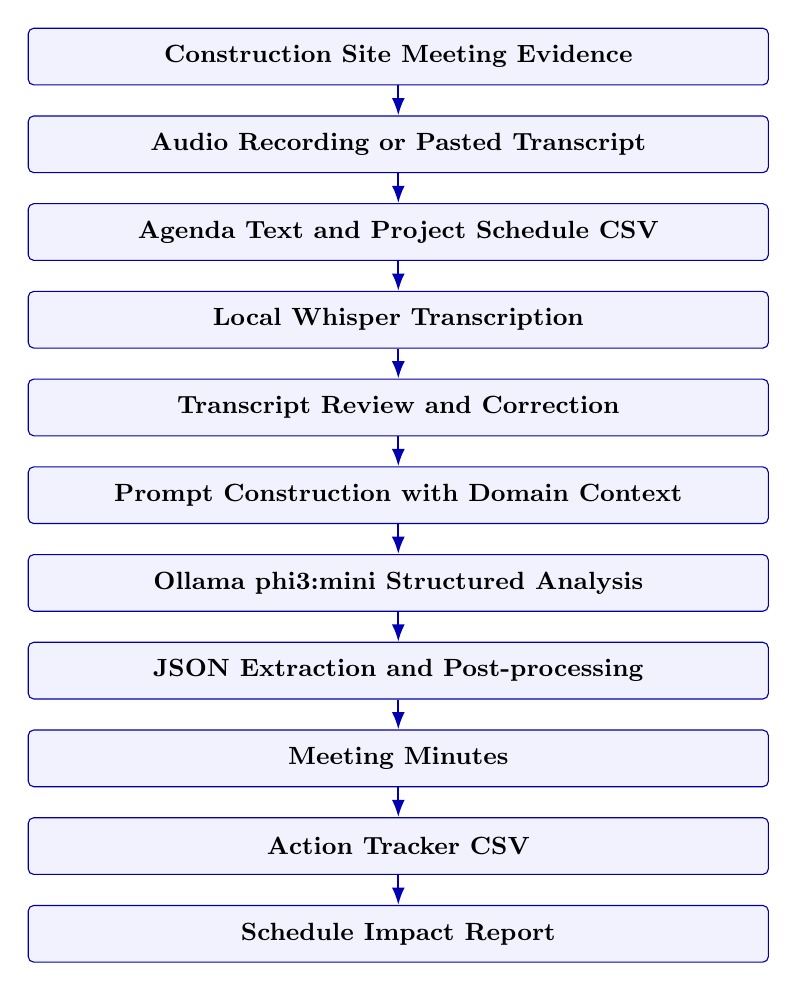
\begin{tikzpicture}[
    node distance=0.38cm,
    process/.style={draw=blue!65!black, rounded corners=2pt, fill=blue!5, align=center, minimum width=9.4cm, minimum height=0.72cm, text width=9.1cm, font=\small\bfseries},
    arrow/.style={-{Latex[length=2.2mm]}, thick, draw=blue!70!black}
]
\node[process] (a) {Construction Site Meeting Evidence};
\node[process, below=of a] (b) {Audio Recording or Pasted Transcript};
\node[process, below=of b] (c) {Agenda Text and Project Schedule CSV};
\node[process, below=of c] (d) {Local Whisper Transcription};
\node[process, below=of d] (e) {Transcript Review and Correction};
\node[process, below=of e] (f) {Prompt Construction with Domain Context};
\node[process, below=of f] (g) {Ollama phi3:mini Structured Analysis};
\node[process, below=of g] (h) {JSON Extraction and Post-processing};
\node[process, below=of h] (i) {Meeting Minutes};
\node[process, below=of i] (j) {Action Tracker CSV};
\node[process, below=of j] (k) {Schedule Impact Report};
\foreach \x/\y in {a/b,b/c,c/d,d/e,e/f,f/g,g/h,h/i,i/j,j/k}
    \draw[arrow] (\x) -- (\y);
\end{tikzpicture}
\caption{Workflow of the proposed local AI-based construction site meeting intelligence system.}
\end{figure}

\subsection{Input Acquisition}

The system accepts four categories of input. The first is an audio recording of the site meeting. The second is transcript text, which may be pasted directly if the meeting has already been transcribed. The third is the meeting agenda, which lists expected discussion points. The fourth is a project schedule CSV containing activities, owners, planned dates or status information.

This input design is important because meeting understanding improves when the model has context. If the agenda states that concrete curing, material delivery and safety inspection must be discussed, the system can identify which agenda points were covered and which were missed. If the schedule contains linked activities, the system can flag possible impacts from blockers or delays mentioned in the meeting.

\subsection{Whisper Transcription}

When an audio file is uploaded, the frontend sends it to the Flask Whisper server. The server exposes routes for health checking, model warmup and automatic speech recognition. Supported audio formats include common meeting recording formats such as MP3, WAV, M4A and WebM. After transcription, the server returns text to the frontend. The transcript is not hidden from the user; it is placed in an editable field so that errors can be corrected before analysis.

The editable transcript step is a practical safeguard. A construction meeting may contain names of local contractors, site blocks, material brands, tower numbers or abbreviations. If the speech recognizer mishears any of these terms, direct LLM analysis may produce incorrect action items. Human review between transcription and analysis reduces this risk.

\subsection{Agenda Cross-reference}

The agenda cross-reference stage compares the meeting content with the expected agenda items. The system asks the model to determine which agenda topics were discussed, which were partially discussed and which were missed. This feature is valuable because a meeting summary alone cannot tell whether the meeting achieved its purpose. For example, a meeting may generate a useful summary but still fail to discuss safety inspection or procurement follow-up.

\subsection{Structured LLM Analysis}

The LLM analysis stage uses a carefully prepared prompt. The prompt instructs the model to behave like a construction meeting assistant and return machine-readable JSON. The required fields include meeting summary, decisions, blockers, action items, risks, agenda coverage and schedule impact. The prompt also asks for owners, due dates and priority where available. If the information is not present, the model should use an empty value rather than inventing details.

The output is parsed by the frontend. If the model produces extra text around the JSON, the application attempts to extract the JSON block. The parsed structure is then rendered into sections of the dashboard. This approach makes the output more useful than free-form text because each field can be displayed, exported and reviewed separately.

\subsection{Schedule Impact Analysis}

The schedule CSV is used to identify whether meeting statements may affect project activities. If the meeting mentions a delay in cement delivery and the schedule contains concreting tasks, the system can mark a potential schedule impact. The current implementation is a Version 1 rule-supported and LLM-supported analysis, not a full critical path scheduling engine. Its purpose is to flag possible impacts early so that the engineer can review them.

\section{System Architecture and Implementation}

The system architecture has four main layers: frontend layer, speech layer, model layer and output layer. The frontend is implemented using HTML, CSS and JavaScript. It manages file upload, transcript editing, agenda entry, schedule upload and result rendering. The speech layer is implemented as a Flask server running on localhost. The model layer uses Ollama on localhost with phi3:mini. The output layer renders meeting minutes, action tracker tables and schedule impact information.

\begin{figure}[H]
\centering
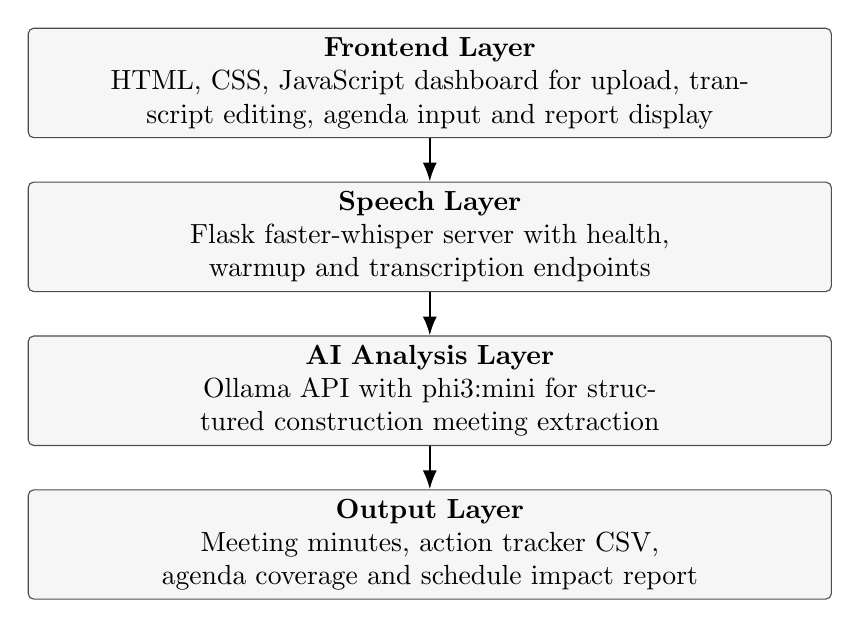
\begin{tikzpicture}[
    layer/.style={draw=black!70, rounded corners=2pt, fill=gray!7, align=center, minimum width=10.2cm, minimum height=1.05cm, text width=9.8cm},
    arrow/.style={-{Latex[length=2.4mm]}, thick}
]
\node[layer] (front) {\textbf{Frontend Layer}\\HTML, CSS, JavaScript dashboard for upload, transcript editing, agenda input and report display};
\node[layer, below=0.55cm of front] (speech) {\textbf{Speech Layer}\\Flask faster-whisper server with health, warmup and transcription endpoints};
\node[layer, below=0.55cm of speech] (model) {\textbf{AI Analysis Layer}\\Ollama API with phi3:mini for structured construction meeting extraction};
\node[layer, below=0.55cm of model] (output) {\textbf{Output Layer}\\Meeting minutes, action tracker CSV, agenda coverage and schedule impact report};
\draw[arrow] (front) -- (speech);
\draw[arrow] (speech) -- (model);
\draw[arrow] (model) -- (output);
\end{tikzpicture}
\caption{Layered architecture of Site Meeting Copilot v2.}
\end{figure}

\subsection{Frontend Dashboard}

The frontend provides the main user interface. It allows the user to upload an audio file, paste transcript text, enter meeting agenda and upload a schedule CSV. After analysis, the dashboard displays the generated output in separate sections. This separation helps the user quickly inspect decisions, blockers, tasks and schedule risks rather than reading a long unstructured paragraph.

The interface also supports export operations. Meeting minutes can be saved as a document-style output, action items can be exported as CSV and schedule impact can be reviewed separately. These exports support practical academic demonstration because the output can be submitted as evidence of system functionality.

\subsection{Whisper Server}

The Whisper server is implemented in Python using Flask. It provides a health endpoint to confirm whether the server is running, a warmup endpoint to load the model and an ASR endpoint to transcribe uploaded audio. Keeping this server separate from the frontend makes the architecture easier to evolve. A future backend can reuse the same speech service or replace it with a more scalable speech pipeline.

\subsection{Ollama Integration}

The frontend communicates with Ollama through the local API. The prompt contains the meeting transcript, agenda and schedule summary. The model is asked to return a JSON object following the expected structure. Since small local models may not always return perfect JSON, the application includes logic to locate and parse the JSON portion of the response. This design is a reasonable Version 1 approach for a student MVP, but production systems should use stricter schema validation and stronger models.

\subsection{Output Generation}

The generated outputs are divided into meeting intelligence categories. The summary explains the overall meeting. Decisions record what was approved or agreed. Blockers identify constraints preventing progress. Action items include owner and due date when available. Agenda coverage shows what was discussed and missed. Schedule impact identifies project activities that may be affected. This output design converts meeting evidence into a project control artifact.

\begin{table}[H]
\centering
\caption{Inputs, processing methods and generated outputs in the Version 1 system.}
\begin{tabularx}{\textwidth}{p{3.2cm}Y Y}
\toprule
\textbf{Input Evidence} & \textbf{Processing Method} & \textbf{Generated Output} \\
\midrule
Meeting audio & Local Whisper transcription through Flask server & Editable transcript for user review \\
Transcript text & Prompt construction and LLM analysis & Summary, decisions, blockers and risks \\
Meeting agenda & Agenda cross-reference with transcript & Discussed, partially discussed and missed agenda items \\
Schedule CSV & Schedule parsing and impact detection & Possible schedule impact report \\
LLM JSON response & JSON extraction and dashboard rendering & Minutes, action tracker and exportable records \\
\bottomrule
\end{tabularx}
\end{table}

\section{Version 1 Release Requirement Mapping}

The Version 1 release is defined as a construction meeting intelligence MVP. It must prove that the system can accept meeting evidence, convert audio to transcript, analyse the content and generate structured outputs. Table \ref{tab:reqmap} maps the implemented functions to the release requirements.

\begin{table}[H]
\centering
\caption{Version 1 requirement mapping for Site Meeting Copilot v2.}
\label{tab:reqmap}
\begin{tabularx}{\textwidth}{p{3.4cm}Y p{2.2cm}}
\toprule
\textbf{Requirement} & \textbf{Implementation in Project} & \textbf{Status} \\
\midrule
Audio upload support & Frontend accepts supported audio files and sends them to the Whisper server & Implemented \\
Speech transcription & Flask server uses faster-whisper to transcribe uploaded audio & Implemented \\
Transcript editing & User can review and modify transcript before analysis & Implemented \\
Agenda support & User can enter agenda text for cross-reference & Implemented \\
Schedule CSV support & User can upload project schedule CSV for impact context & Implemented \\
Meeting summary & LLM extracts concise meeting summary & Implemented \\
Decision extraction & LLM identifies decisions from transcript & Implemented \\
Blocker extraction & LLM identifies blockers and risks & Implemented \\
Action tracker & LLM extracts tasks, owners and deadlines where available & Implemented \\
Schedule impact report & System flags possible schedule-related impacts & Implemented \\
Export support & Dashboard supports output export for minutes and trackers & Implemented \\
Local operation & Uses local Whisper server and local Ollama model & Implemented \\
\bottomrule
\end{tabularx}
\end{table}

The mapping shows that the current project satisfies the core Version 1 requirements. The release is not a full enterprise system because it does not yet include authentication, persistent database storage, project-level memory or multi-user roles. However, those features belong to future versions. The Version 1 goal is to convert site meeting evidence into structured and reviewable records, and that goal is achieved.

\section{Algorithmic Workflow}

The algorithmic workflow begins with input collection and ends with report generation. The simplified workflow is shown below.

\begin{verbatim}
Input:
    audio_file OR transcript_text
    agenda_text
    schedule_csv

Process:
    if audio_file is provided:
        transcript = whisper_server.transcribe(audio_file)
    else:
        transcript = transcript_text

    user reviews transcript
    schedule_context = parse_schedule(schedule_csv)
    prompt = build_prompt(transcript, agenda_text, schedule_context)
    raw_response = ollama.generate(model="phi3:mini", prompt=prompt)
    json_result = extract_json(raw_response)
    dashboard.render(json_result)

Output:
    meeting_minutes
    decision_log
    blocker_list
    action_tracker
    agenda_coverage
    schedule_impact_report
\end{verbatim}

The most important part of the workflow is the structured analysis stage. The prompt is designed to reduce hallucination by asking the model to use only the meeting evidence and context. If information is missing, the model should leave the field empty or mark it as not specified. This is important in construction because assigning an incorrect owner or due date may create confusion in the project team.

\section{Evaluation Design}

The system was evaluated as a functional Version 1 prototype. The objective of evaluation was not to benchmark against enterprise software, but to verify whether each required workflow can be completed. The tests were designed around expected use by an engineering student demonstrating the project.

\subsection{Test Environment}

The prototype runs locally on a Windows development machine. The frontend runs in the browser using local project files. Ollama runs on localhost port 11434 and provides phi3:mini inference. The Whisper server runs as a local Flask application on localhost port 9000. The project includes a sample schedule CSV for demonstration and validation.

\subsection{Functional Test Cases}

The functional tests included frontend loading, schedule CSV upload, audio upload route availability, Whisper health endpoint, transcript analysis, malformed schedule handling and export output checking. Table \ref{tab:functional} summarizes the major tests.

\begin{table}[H]
\centering
\caption{Functional evaluation summary.}
\label{tab:functional}
\begin{tabularx}{\textwidth}{p{3.2cm}Y p{2.6cm}}
\toprule
\textbf{Test Area} & \textbf{Expected Behaviour} & \textbf{Result} \\
\midrule
Frontend load & Application opens and displays meeting input fields & Passed \\
Audio upload interface & User can select supported meeting audio files & Passed \\
Whisper health route & Server confirms availability before transcription & Passed \\
Transcript handling & Transcript can be pasted or filled from ASR output & Passed \\
Agenda analysis & Agenda points are compared against transcript content & Passed \\
Schedule CSV handling & Valid CSV is parsed and malformed CSV is handled gracefully & Passed \\
LLM analysis & Model returns structured meeting intelligence categories & Passed with review needed \\
JSON extraction & Application extracts usable JSON from model response & Passed \\
Output display & Dashboard renders summary, decisions, blockers and tasks & Passed \\
Export output & Reports and tracker outputs are available for submission & Passed \\
\bottomrule
\end{tabularx}
\end{table}

\subsection{Evaluation Observations}

The evaluation showed that the workflow is suitable for a Version 1 construction meeting intelligence prototype. The most useful outputs are action items and blockers because they directly support follow-up after the meeting. Agenda coverage is also valuable because it shows whether the meeting actually addressed planned discussion points. Schedule impact is useful as an early warning signal, but it should be treated as advisory in the current version.

The evaluation also showed the importance of transcript review. If a meeting recording is noisy, transcription errors can affect the LLM output. Human correction before analysis improves reliability. This confirms the design decision to keep the transcript visible and editable.

\section{Results and Discussion}

\subsection{Meeting Intelligence}

The strongest result of the project is meeting intelligence extraction. The system can transform a transcript into categories that are useful for project management. Instead of returning a generic summary, it extracts decisions, blockers, action items, owners, deadlines and risks. This matches a real construction need because site teams require follow-up records, not only prose summaries.

For example, if a meeting discussion states that electrical conduits are delayed because the supplier has not delivered material, the system can identify the supplier issue as a blocker, create an action item for follow-up and mark related electrical work as a schedule risk. This type of structured transformation is the main value of the project.

\subsection{Agenda Coverage}

Agenda coverage is a distinctive feature compared with normal meeting summarization tools. A meeting can be long and still miss a critical agenda item. By asking the AI to identify covered and missed points, the system helps the user check meeting completeness. This feature is especially useful for project review meetings, where safety, procurement, labour and schedule must all be addressed.

\subsection{Schedule Impact}

Schedule impact analysis moves the system closer to construction project management. The current version does not calculate a formal critical path, but it identifies risks that may affect scheduled tasks. This is suitable for Version 1 because it provides early warning without claiming to replace professional scheduling software.

\subsection{Local-first Design}

The local-first design is suitable for academic demonstration and early prototyping. Running Whisper and Ollama locally reduces dependence on paid APIs and supports privacy. It also allows the student to demonstrate the system in a lab environment. However, local models may be slower or less accurate than stronger cloud models. Therefore, the future production roadmap may include optional cloud inference while keeping local processing as a privacy-friendly mode.

\subsection{Human Review}

The system is intentionally designed for human review. It does not automatically send messages, update schedules or assign tasks without user approval. This is important because meeting records may have contractual and operational consequences. A site engineer should verify the output before sharing it with the team.

\section{Limitations}

The Version 1 implementation has several limitations. First, transcription accuracy depends on audio quality. Construction site recordings may include background noise, overlapping speakers and technical terms. Second, phi3:mini is a compact local model and may sometimes produce incomplete or imperfect JSON. Third, the system does not yet include speaker diarization, so it may not always identify who said what. Fourth, project history is not stored in a database, so the system cannot yet answer long-term questions across many meetings.

Another limitation is that schedule impact analysis is advisory rather than computationally complete. The system can flag possible impacts, but it does not calculate the critical path or update a professional project schedule. The schedule CSV format must also be reasonably structured for reliable parsing. These limitations are acceptable for Version 1 but should be addressed in future versions.

\section{Future Scope}

The future roadmap can evolve Site Meeting Copilot v2 into a broader construction AI assistant. The first major upgrade is a backend architecture using React or Next.js for the frontend, FastAPI for the backend and PostgreSQL for persistent storage. This would allow users, projects, meetings, transcripts, tasks and decisions to be stored securely.

The second upgrade is project memory. Instead of analysing one meeting at a time, the system should store meeting transcripts, documents, schedules, photographs and task histories. A user could then ask questions such as, ``Why is Tower B delayed?'' The system could search past meetings, schedule entries and action items to produce an evidence-based answer.

The third upgrade is an agent-based architecture. Separate agents could handle meetings, schedules, documents and vendor follow-ups. A construction manager agent could coordinate their outputs and recommend actions. For example, the meeting agent could identify unresolved issues, the schedule agent could detect delay risk and the document agent could compare the issue with contract requirements.

The fourth upgrade is controlled action execution. After human approval, the system could create tasks, notify responsible persons and update project status. This would transform the tool from a meeting analyser into an AI-supported project management system. However, approvals and audit logs would be essential because construction actions affect cost, safety and responsibility.

\section{Conclusion}

This paper presented Site Meeting Copilot v2, a local AI-based framework for construction site meeting intelligence. The system accepts audio or transcript input, uses Whisper transcription, analyses meeting content with a local language model, checks agenda coverage and flags schedule impacts. It then exports meeting minutes, an action tracker and a schedule impact report.

The Version 1 implementation satisfies the main requirements of a construction meeting minutes and action tracker MVP. It demonstrates how local AI tools can help site engineers convert unstructured meeting evidence into structured and reviewable project records. The project is not yet a full construction AI operating system, but it provides a strong foundation. Future work should add a backend, database storage, authentication, project memory, speaker diarization and specialized agents for meetings, schedules and documents.

\newpage

\section*{Appendix A: Example Structured Output Schema}

The following schema represents the type of structured output expected from the language model. In the implementation, the exact JSON may vary depending on transcript content, but the categories remain consistent.

\begin{verbatim}
{
  "summary": "Brief meeting summary",
  "decisions": [
    {
      "decision": "Decision text",
      "owner": "Responsible person if mentioned",
      "evidence": "Transcript phrase supporting the decision"
    }
  ],
  "blockers": [
    {
      "blocker": "Issue preventing progress",
      "impact": "Affected work or project area",
      "priority": "Low, Medium or High"
    }
  ],
  "action_items": [
    {
      "task": "Action to be completed",
      "owner": "Assigned person",
      "due_date": "Deadline if mentioned",
      "status": "Pending"
    }
  ],
  "agenda_coverage": {
    "discussed": ["Agenda items discussed"],
    "missed": ["Agenda items not discussed"]
  },
  "schedule_impact": [
    {
      "activity": "Schedule activity affected",
      "risk": "Reason for possible impact",
      "severity": "Low, Medium or High"
    }
  ]
}
\end{verbatim}

\section*{Appendix B: Demonstration Workflow}

The recommended demonstration workflow is as follows:

\begin{enumerate}[leftmargin=0.6cm]
    \item Start Ollama and confirm that the phi3:mini model is available.
    \item Start the Whisper server and check the health endpoint.
    \item Open the Site Meeting Copilot v2 frontend in the browser.
    \item Upload a sample meeting audio file or paste a transcript.
    \item Enter the meeting agenda.
    \item Upload the sample project schedule CSV.
    \item Run the meeting analysis.
    \item Review the generated summary, decisions, blockers, action items and schedule impacts.
    \item Export the meeting minutes and action tracker.
    \item Explain how this Version 1 system can evolve into a construction AI project manager.
\end{enumerate}

\section*{Appendix C: Research Relevance}

The research relevance of this project is that it connects speech recognition, local language models and construction project control. Many AI meeting tools focus on generic summarization. This project demonstrates that domain-specific meeting intelligence can be more useful when it produces structured project management outputs. The construction domain is suitable for this approach because meetings are frequent, decisions are time-sensitive and delays can propagate through schedules.

The framework also supports responsible AI use. It does not hide the transcript, and it does not automatically execute decisions. It presents AI-generated outputs for human review. This is important in construction, where records may affect safety, cost and accountability. The project therefore balances automation with professional oversight.

\begin{thebibliography}{99}

\bibitem{whisper}
A. Radford, J. W. Kim, T. Xu, G. Brockman, C. McLeavey and I. Sutskever, ``Robust speech recognition via large-scale weak supervision,'' in \textit{Proceedings of the International Conference on Machine Learning}, 2023. Available: \url{https://arxiv.org/abs/2212.04356}

\bibitem{fasterwhisper}
SYSTRAN, ``faster-whisper: Transcription with CTranslate2,'' GitHub repository. Available: \url{https://github.com/SYSTRAN/faster-whisper}

\bibitem{phi3}
M. Abdin et al., ``Phi-3 technical report: A highly capable language model locally on your phone,'' arXiv, 2024. Available: \url{https://arxiv.org/abs/2404.14219}

\bibitem{ollama}
Ollama, ``Generate a response API documentation.'' Available: \url{https://docs.ollama.com/api/generate}

\bibitem{constructionmeetings}
R. Ludwig, ``Meetings critical to construction project success and best practices: A case study,'' California Polytechnic State University, 2018. Available: \url{https://digitalcommons.calpoly.edu/cmsp/183}

\bibitem{constructionmanagement}
P. Fewings and C. Henjewele, \textit{Construction Project Management: An Integrated Approach}, 3rd ed. Routledge, 2019.

\bibitem{projectmanagement}
Project Management Institute, \textit{A Guide to the Project Management Body of Knowledge}, 7th ed. Project Management Institute, 2021.

\bibitem{localai}
K. Lokaditya, ``Site Meeting Copilot v2 project implementation and final report,'' Dayananda Sagar University, Bengaluru, India, 2026.

\end{thebibliography}

\end{document}
